\documentclass[tikz]{standalone}
\usepackage{tikz}
\usetikzlibrary{shapes.geometric, arrows.meta, positioning, fit}

\begin{document}

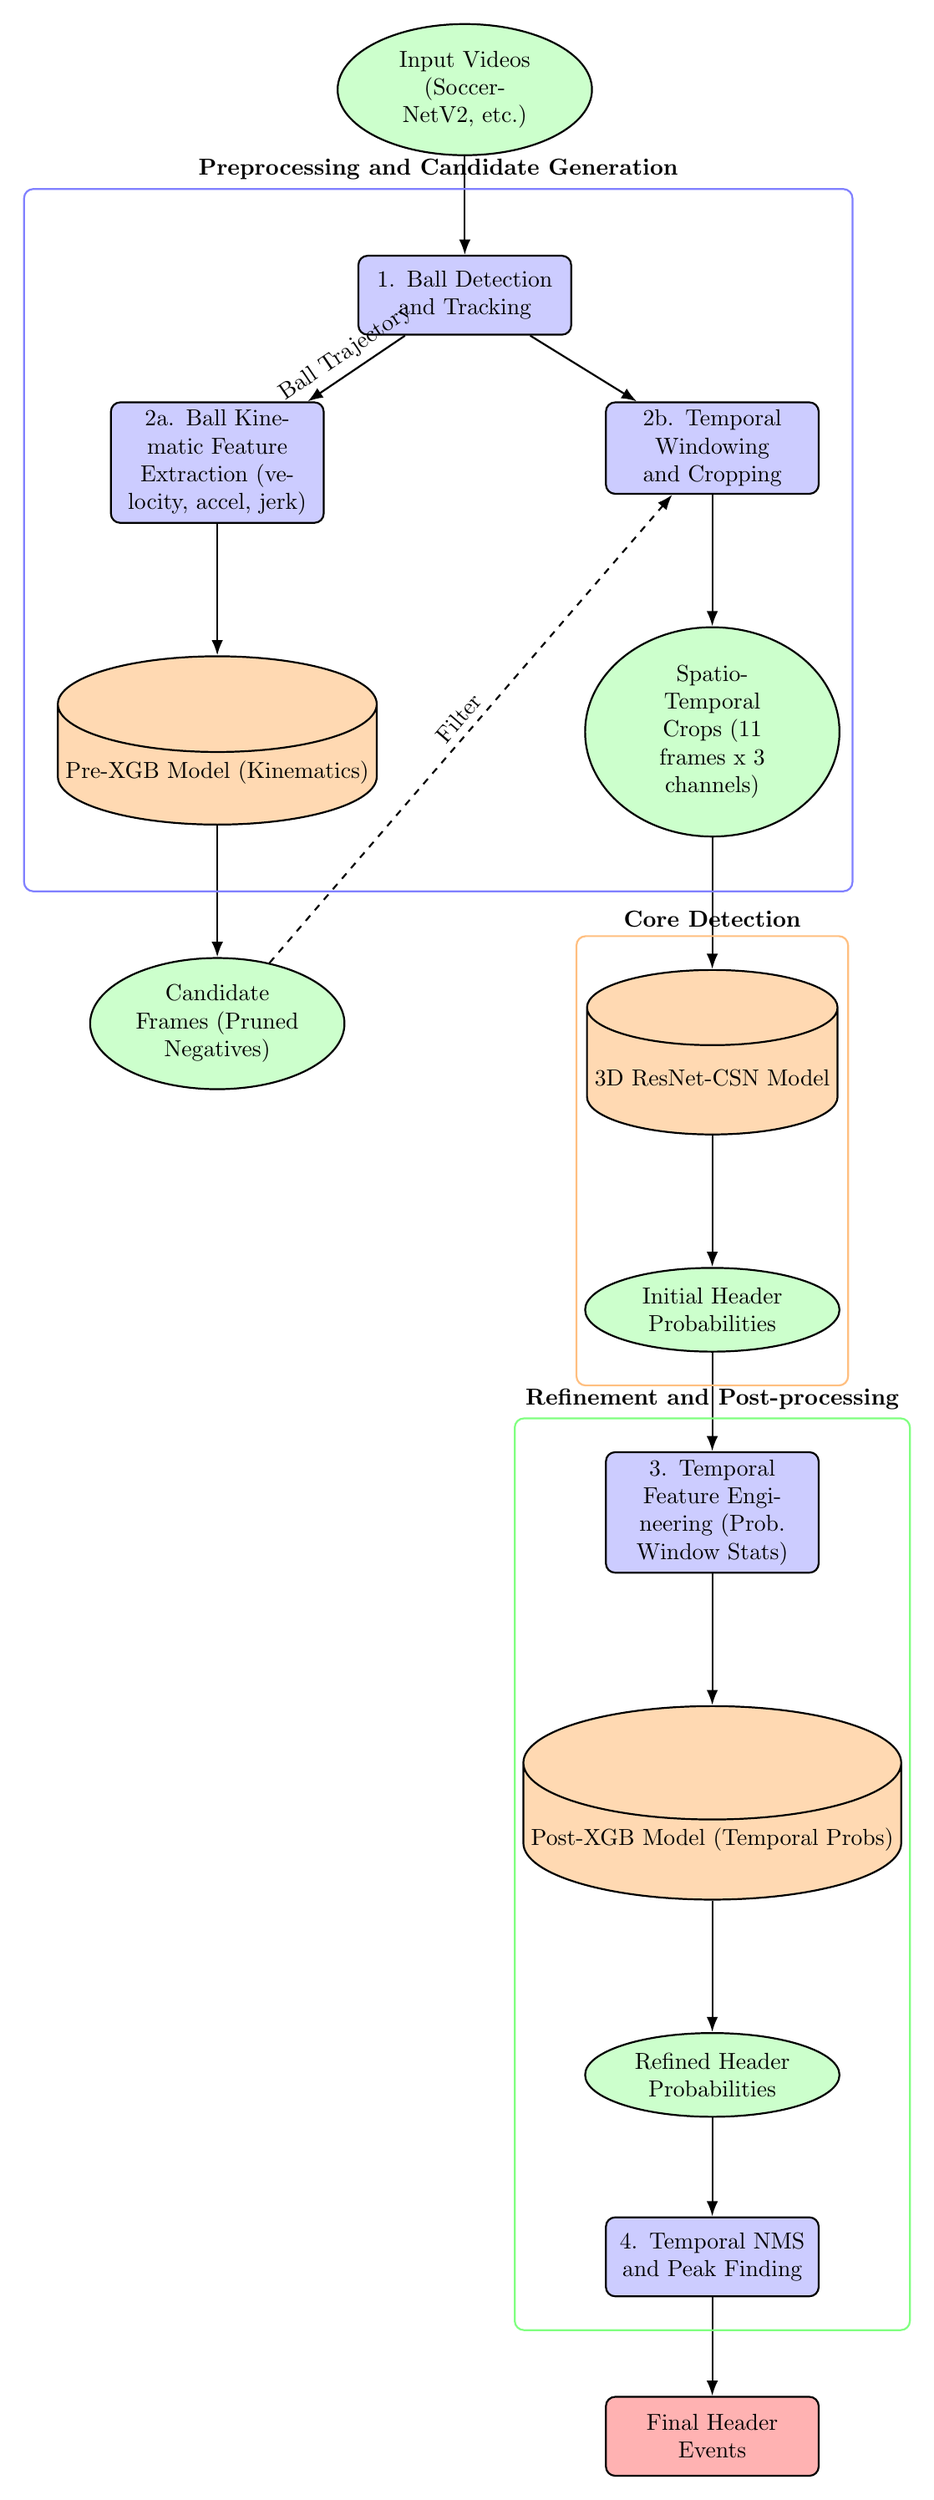
\begin{tikzpicture}[
    node distance=1.5cm and 2cm,
    process/.style={rectangle, rounded corners, minimum width=3cm, minimum height=1.2cm, text centered, text width=3cm, draw=black, fill=blue!20, thick},
    data/.style={ellipse, minimum width=2.5cm, text centered, text width=2.5cm, draw=black, fill=green!20, thick},
    model/.style={cylinder, shape border rotate=90, aspect=0.3, minimum height=2.5cm, minimum width=1.5cm, text centered, draw=black, fill=orange!30, thick},
    final/.style={rectangle, rounded corners, minimum width=3cm, minimum height=1.2cm, text centered, text width=3cm, draw=black, fill=red!30, thick},
    arrow/.style={-Latex, thick},
    dashed_arrow/.style={-Latex, thick, dashed},
    % Style for the bounding box labels
    stage_label/.style={font=\bfseries}
]

% STAGE 1: Data Input & Preprocessing
\node (videos) [data] {Input Videos (SoccerNetV2, etc.)};
\node (ball_det) [process, below=of videos] {1. Ball Detection and Tracking};
\node (kinematics) [process, below left=1cm and 0.5cm of ball_det] {2a. Ball Kinematic Feature Extraction (velocity, accel, jerk)};
\node (sampling) [process, below right=1cm and 0.5cm of ball_det] {2b. Temporal Windowing and Cropping};

% STAGE 2: Weak Prefilter (XGB)
\node (pre_xgb) [model, below=of kinematics, yshift=-0.5cm] {Pre-XGB Model (Kinematics)};
\node (candidates) [data, below=of pre_xgb, yshift=-0.5cm] {Candidate Frames (Pruned Negatives)};

% STAGE 3: Main Detection Model (CNN)
\node (cnn_input) [data, below=of sampling, yshift=-0.5cm] {Spatio-Temporal Crops (11 frames x 3 channels)};
\node (cnn_model) [model, below=of cnn_input, yshift=-0.5cm] {3D ResNet-CSN Model};
\node (cnn_probs) [data, below=of cnn_model, yshift=-0.5cm] {Initial Header Probabilities};

% STAGE 4: Refinement (XGB)
\node (temporal_feats) [process, below=of cnn_probs] {3. Temporal Feature Engineering (Prob. Window Stats)};
\node (post_xgb) [model, below=of temporal_feats, yshift=-0.5cm] {Post-XGB Model (Temporal Probs)};
\node (final_probs) [data, below=of post_xgb, yshift=-0.5cm] {Refined Header Probabilities};

% STAGE 5: Final Event Detection
\node (nms) [process, below=of final_probs] {4. Temporal NMS and Peak Finding};
\node (output) [final, below=of nms] {Final Header Events};

% Arrows
\draw [arrow] (videos) -- (ball_det);
\draw [arrow] (ball_det) -- node[pos=0.5, above, sloped] {Ball Trajectory} (kinematics);
\draw [arrow] (ball_det) -- (sampling);

\draw [arrow] (kinematics) -- (pre_xgb);
\draw [arrow] (pre_xgb) -- (candidates);
\draw [dashed_arrow] (candidates) -- node[pos=0.5, above, sloped] {Filter} (sampling);

\draw [arrow] (sampling) -- (cnn_input);
\draw [arrow] (cnn_input) -- (cnn_model);
\draw [arrow] (cnn_model) -- (cnn_probs);

\draw [arrow] (cnn_probs) -- (temporal_feats);
\draw [arrow] (temporal_feats) -- (post_xgb);
\draw [arrow] (post_xgb) -- (final_probs);

\draw [arrow] (final_probs) -- (nms);
\draw [arrow] (nms) -- (output);

% Bounding Boxes for conceptual stages
\node[draw=blue!50, thick, rounded corners, inner ysep=1cm, inner xsep=0.5cm, fit=(ball_det) (kinematics) (sampling) (pre_xgb), label={[stage_label]above:Preprocessing and Candidate Generation}] {};
\node[draw=orange!50, thick, rounded corners, inner ysep=0.5cm, fit=(cnn_model) (cnn_probs), label={[stage_label]above:Core Detection}] {};
\node[draw=green!50, thick, rounded corners, inner ysep=0.5cm, fit=(temporal_feats) (post_xgb) (nms), label={[stage_label]above:Refinement and Post-processing}] {};

\end{tikzpicture}

\end{document}